\documentclass[dvipdfmx,10pt]{jlreq}
\usepackage[top=30truemm,bottom=30truemm,left=15truemm,right=15truemm]{geometry}
\usepackage{graphicx}
\usepackage{tikz-qtree}

\begin{document}

\title{第11回 予習復習問題}
\author{2025311066 藤井壮樹}
\date{\today}
\maketitle

\section{第9回予習復習問題の確認・修正}
\subsection*{1.}
確認しました.
\subsection*{2.}
確認しました.
\subsection*{3.}
確認しました.
\subsection*{4.}
確認しました.
\newpage
\section{第11回予習復習問題}
\subsection*{5.}
\begin{figure}
\centering
\includegraphics[width=0.8\textwidth]{flow11.jpg}
\caption{フローチャート}
\end{figure}
\subsection*{6.}
\begin{itemize}
\item まずは,二分探索と同じように要素を挿入する.
\item 平衡係数を計算し,それに基づいてLR回転を行う.
\end{itemize}
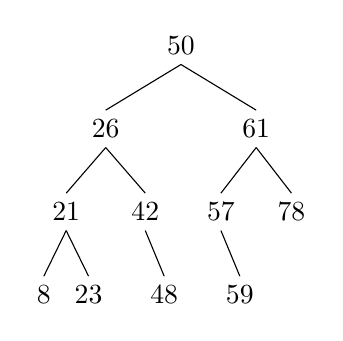
\begin{tikzpicture}
\tikzset{every tree node/.style={align=center,anchor=north}}
\Tree
[.50
    [.26
        [.21
            [.8 ]
            [.23 ]
        ]
        [.42
            \edge[draw=none]; \node[draw=none]{}; % 左側が空の場合
            [.48 ]
        ]
    ]
    [.61
        [.57 
            \edge[draw=none]; \node[draw=none]{}; 
            [.59 ]
        ]
        [.78 ]
    ]
]
\end{tikzpicture}



%\begin{thebibliography}{}
%	\bibitem{文献1}
%\end{thebibliography}

\end{document}